\chapter{Experiments}
\label{ch2}

\section{CMS experiment}

The CMS is a detector that consist on different detectors made for detecting different particles, like the silicon tracker, the electromagnetic calorimeter, the hadron calorimeter the superconducting solenoid and the muon chamber. Its a cylindrical onion with several  \cite{CMS}

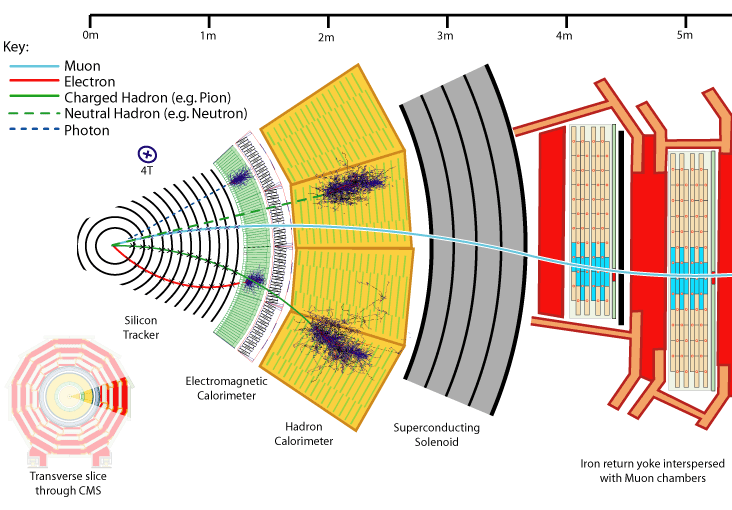
\includegraphics[scale=0.35]{cms.png}

\section{Pixel Detector}

This is one of the detectors of the CMS \cite{pxd}

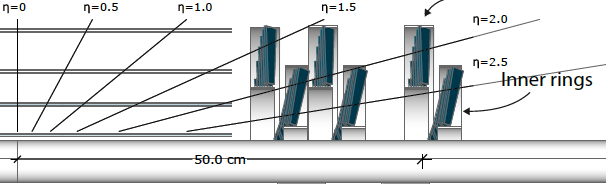
\includegraphics[scale=0.7]{pixeldetector.png}

\section{PCC method}

The Pixel Cluster Counting (PCC) method


\section{Van Der Meer Method}

The Van Der Meer Method \cite{Vdm}

\section{Calibration Constant}

The calibration constant 

$\sigma_{vis} = \frac{R_{det}}}{L_{b}} = \frac{2 \pi \Sigma_{x} \Sigma_{y} R(0,0)}{N_{1}N_{2}f}$  \cite{Lumvdm}
